\documentclass[a4paper ,12pt, onecolumn]{article}
\usepackage[utf8]{inputenc}
\usepackage[spanish]{babel}
\usepackage[hidelinks]{hyperref}
\usepackage{graphicx}
\begin{document}
\title{Anexo diseño mecánico}

\author{Rubén Arce}
\date{\today}
\maketitle
\cleardoublepage
\tableofcontents
\cleardoublepage

\section{Introducción}
Para llevar a cabo el diseño mecánico de estas piezas concretas se ha optado por emplear Freecad, un
programa de software libre que permite hacer modelos sencillos de forma gratuita.
Se ha empleado la versión 12 del mismo corriendo en una raspberry pi 4 de 4Gb de RAM, es un programa
que consume pocos recursos.
\section{Emisor beacon}
    \subsection{Aspectos a considerar en el diseño}
        \begin{enumerate}
            \item Estéticamente atractivo
            \item Pequeñas dimensiones
        \end{enumerate}
    \subsection{Planos y dimensiones}
    \subsection{Imágenes renderizado}   
        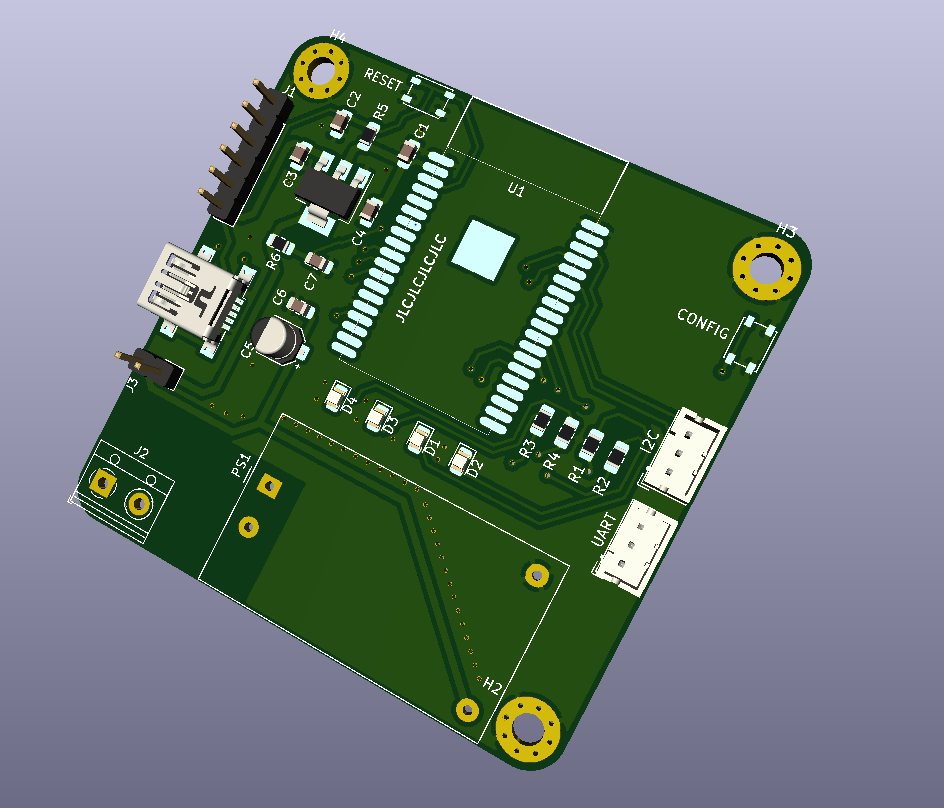
\includegraphics[scale=0.4]{../receiver_1.PNG}
        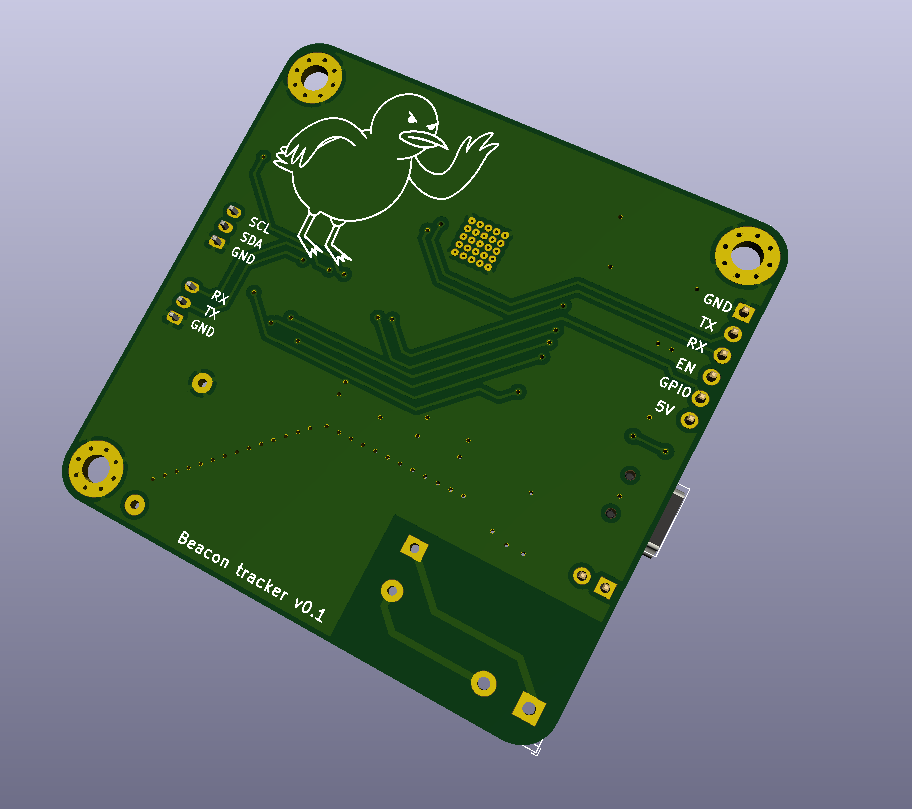
\includegraphics[scale=0.4]{../receiver_2.PNG}
    \subsection{Imágenes reales}
        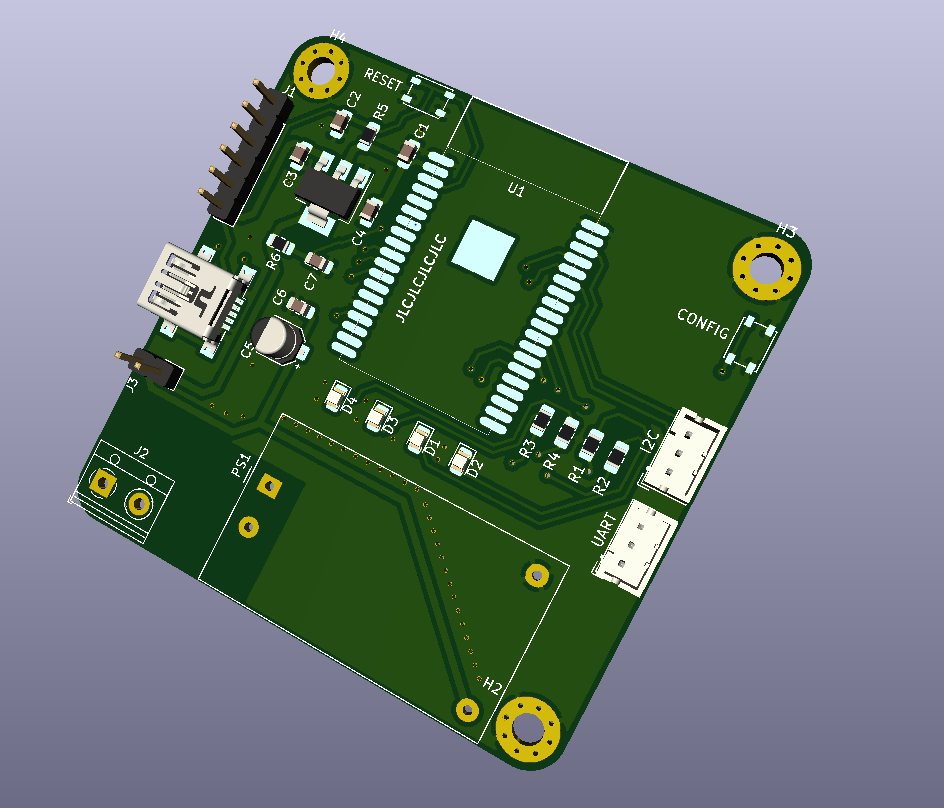
\includegraphics[scale=0.4]{../receiver_1.PNG}
        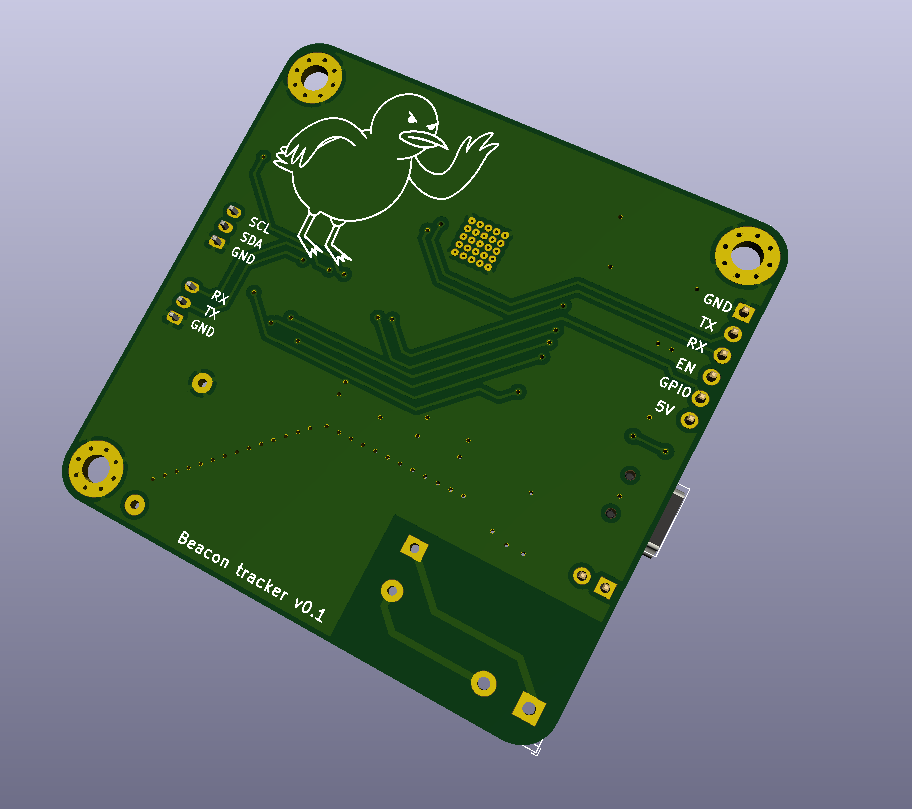
\includegraphics[scale=0.4]{../receiver_2.PNG}

\section{Receptor beacon o gateway}
    \subsection{Aspectos a considerar en el diseño}
        \begin{enumerate}
            \item Estéticamente atractivo
            \item Pequeñas dimensiones
        \end{enumerate}
    \subsection{Planos y dimensiones}
    \subsection{Imágenes renderizado}   
        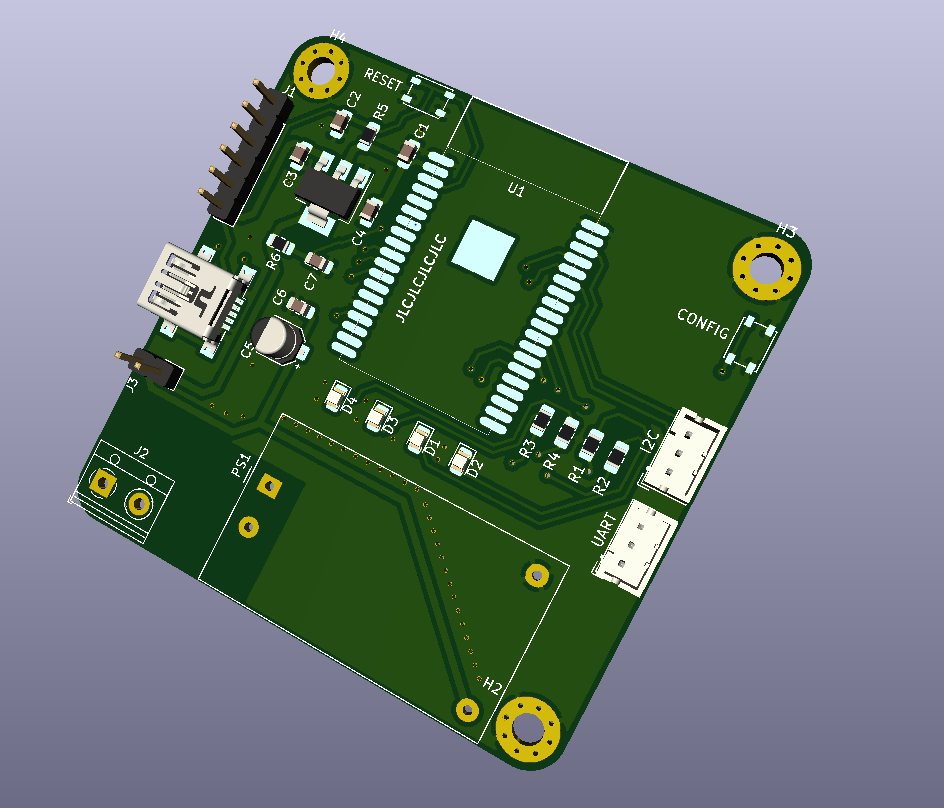
\includegraphics[scale=0.4]{../receiver_1.PNG}
        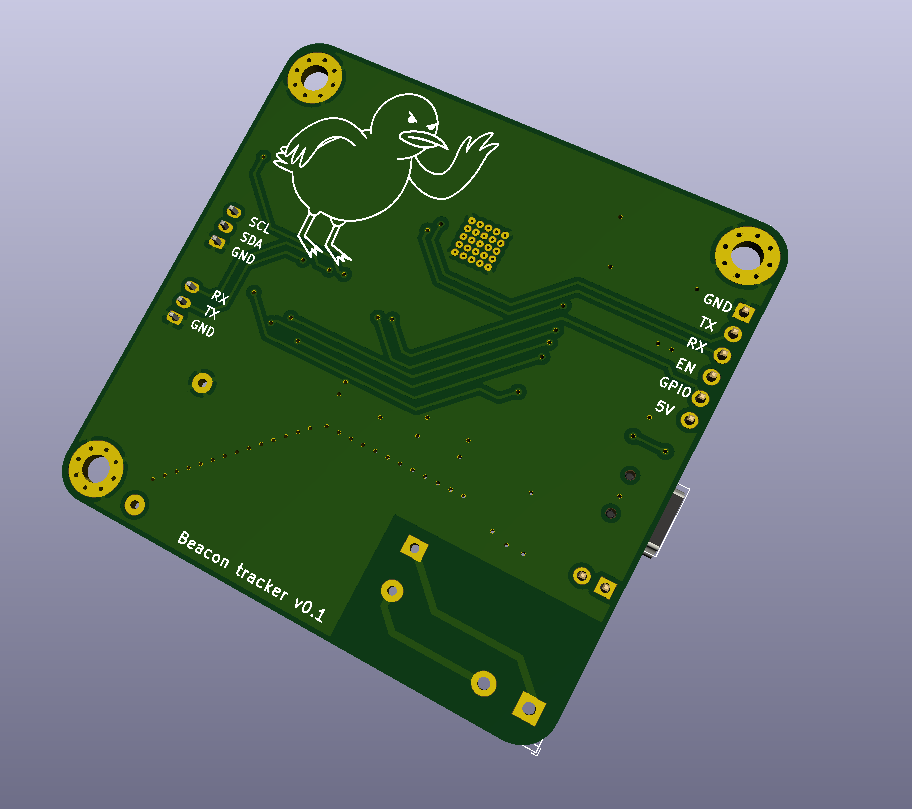
\includegraphics[scale=0.4]{../receiver_2.PNG}
    \subsection{Imágenes reales}
        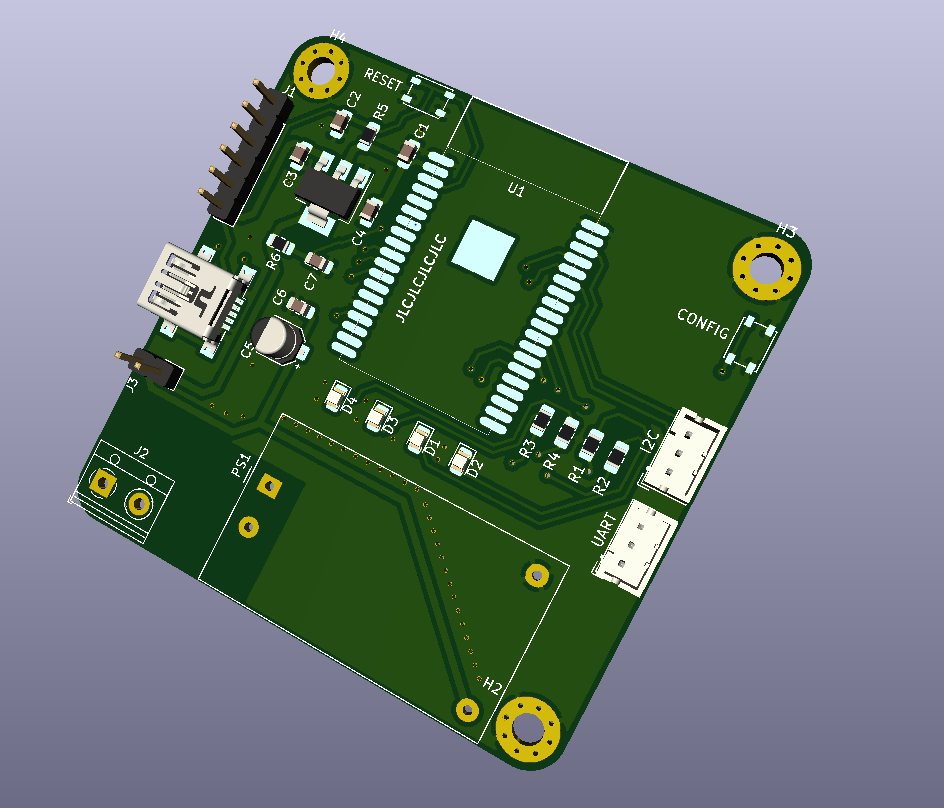
\includegraphics[scale=0.4]{../receiver_1.PNG}
        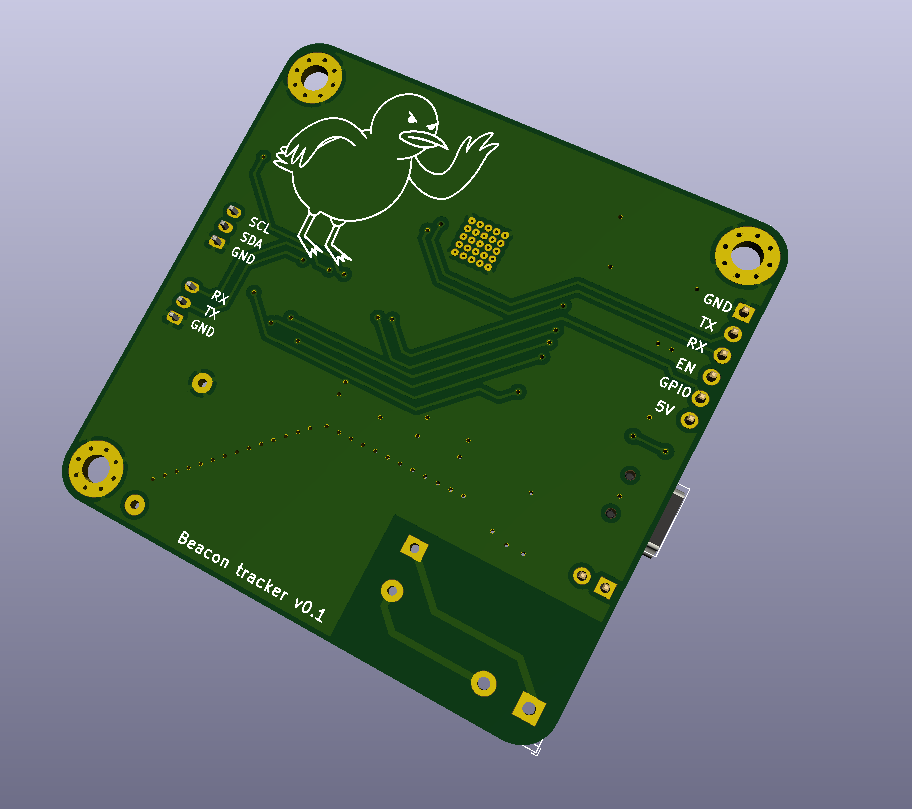
\includegraphics[scale=0.4]{../receiver_2.PNG}

\section{Bibliografía}
https://www.bluetooth.com/
\end{document}